\documentclass[a4paper,12pt]{article} 

%%% Работа с русским языком
\usepackage{cmap}                           % поиск в PDF
\usepackage{mathtext} 			 	       % русские буквы в формулах
\usepackage[T2A]{fontenc}               % кодировка
\usepackage[utf8]{inputenc}              % кодировка исходного текста
\usepackage[english,russian]{babel}  % локализация и переносы
\usepackage{wrapfig}
\usepackage{gensymb}
\usepackage{textcomp}
\usepackage{multirow}
\usepackage{amsmath,amsfonts,amssymb,amsthm,mathtools} % AMS
\usepackage{euscript}	 % Шрифт Евклид
\usepackage{mathrsfs} % Красивый матшрифт
\usepackage{graphicx}%Вставка картинок правильная
\usepackage{float}%"Плавающие" картинки
\usepackage{wrapfig}%Обтекание фигур (таблиц, картинок и прочего)
\title{Лабораторная работа 2.2.3 

Определение теплопроводности воздуха при атмосферном давлении}
\author{Кагарманов Радмир Б01-106}
\date{19 марта 2022 г.}

\begin{document}

\maketitle
\newpage
\paragraph{Цель работы:} измерить коэффициент теплопроводности воздуха при атмосферном давлении в зависимости от температуры.
\paragraph{В работе используется:}цилиндрическая колба с натянутой по оси нитью; термостат; вольтметр; эталонное сопротивление; источник
постоянного напряжения; магазин сопротивлений.

\paragraph{Теоретические сведения \\}

Теплопроводность — это процесс передачи тепловой энергии от нагретых частей системы к холодным за счёт хаотического движения частиц среды.. Перенос тепла описывается законом Фурье, утверждающим, что плотность потока энергии $\Vec{q} [\frac{\text{Вт}}{\text{м}^2}]$ пропорционально градиенту температуры $\nabla T$.

\begin{equation}
    \Vec{q}=-\kappa \cdot \nabla T
\end{equation}
где $\kappa$ - коэффициент теплопроводности. \\

Пусть тонкая нить радиусом $r_1$ и длиной $L$ помещена на оси цилиндра радиусом $r_0$. Температура стенок цилиндра $T_0$ поддерживается постоянной. Пусть в нити выделяется некоторая тепловая мощность $Q$. $r$ - расстояние до оси. Полный поток тепла будет равен $Q=qS$:
\begin{equation}
    Q=-2\pi rL \cdot \kappa \frac{dT}{dr}=const
\end{equation}
Интегрируя от радиуса нити до радиуса колбы, получаем:
\begin{equation}
    Q=\frac{2\pi L }{\text{ln}(\frac{r_0}{r_1})}\kappa \cdot \Delta T
\end{equation}
\paragraph{Экспериментальная установка\\}
Схема установки приведена на рис. 1. На оси
полой цилиндрической трубки с внутренним
диаметром $2r_0$ размещена металлическая нить диаметром $2r_1$ и длиной $L$. Стенки трубки помещены в кожух, через которых пропускается вода из термостата, так что их температура $t_0$ поддерживается постоянной. 
\begin{figure}[h]
    \centering
    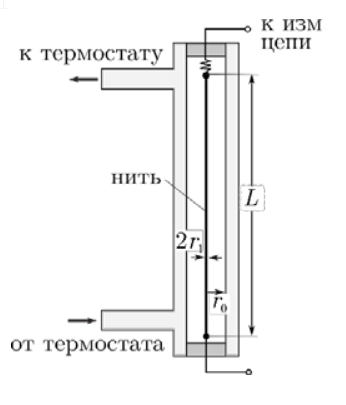
\includegraphics[width=0.5\linewidth]{Установка.png}
    \caption{Экспериментальная установка}
    \label{fig:my_label}
\end{figure}

Металлическая нить служит как источником тепла, так и датчиком температуры (термометром сопротивления). По пропускаемому через нить постоянному току $I$ и напряжению $U$ на ней вычисляется мощность нагрева по закону Джоуля–Ленца:
\begin{equation}
    Q=UI
\end{equation}

На Рис. 2 изображена схема, с помощью которой можно определить сопротивление нити.

\begin{figure}[h]
    \centering
    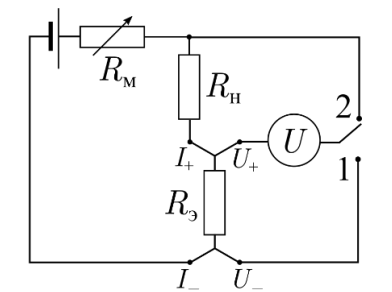
\includegraphics[width=0.5\linewidth]{схема.png}
    \caption{Схема цепи}
    \label{fig:my_label}
\end{figure}
\newpage
\paragraph{Ход работы и обработка результатов \\}
\subparagraph{1.} Параметры установки: \\
$L=365\pm 2 мм$ - длина нити\\
$2r_1=0,055\pm 0,0005мм$ - радиус нити\\
$2r_2=10,0\pm 0,1 мм$ - радиус колбы\\
$R_\text{э}= 10,000 Ом$ - эталонное сопротивление
\subparagraph{2.} Измерим несколько значений тока для различных температур и измерим нагрузочные кривые. В таблице 1 будут результаты этих измерений.
\subparagraph{3.} Сопротивление нити находится по формуле: $R_\text{н} = \frac{U_\text{н}}{U_\text{э}}R_\text{э}$. Мощность $Q = U_\text{н} \cdot \frac{U_\textbf{э}}{R_\text{э}}$.
\subparagraph{4.} Оценим погрешности:
 \begin{center}
     $\sigma Q = Q\sqrt{(\frac{\sigma U_H}{U_H})^2+(\frac{\sigma U_0}{U_0})^2}$
\end{center} \par
\begin{center}
     $\sigma R_\text{н} = R_\text{н}\sqrt{(\frac{\sigma U_H}{U_H})^2+(\frac{\sigma U_0}{U_0})^2}$
\end{center} \par
$\varepsilon_Q= 0,005\%$; $\varepsilon_R = 0,005\%$ 
\subparagraph{5.} Построим для каждой температуры графики зависимости $Q$ от $R_\text{н}$ и определим по ним $\frac{dQ}{dR_\text{н}}$. Они будут изображены на рисунках 3, 4, 5, 6, 7. \\ 
$T_1 = 22,0\degree C: ~ \frac{dQ}{dR_\text{н}}=0,2991;~ R_0=14,548 Ом$ \\
$T_2 = 30,0\degree C: ~ \frac{dQ}{dR_\text{н}}=0,3084;~ R_0=14,938 Ом$ \\
$T_3 = 40,0\degree C: ~ \frac{dQ}{dR_\text{н}}=0,3075;~ R_0=15,344 Ом$ \\
$T_4 = 50,0\degree C: ~ \frac{dQ}{dR_\text{н}}=0,3080;~ R_0=15,815 Ом$ \\
$T_5 = 60,0\degree C: ~ \frac{dQ}{dR_\text{н}}=0,3128;~ R_0=16,272 Ом$
\subparagraph{6.} Построим зависимость $R$ от $t$ и найдём температурный коэффициент молибдена.(Рис.8)
$\alpha =(0,00332 \pm 0,00023) K^{-1}$
Видно, что значение, которое мы получили, не совпадает с табличным $0,004579 K^{-1}$.
\subparagraph{7.} Найдём коэффициент теплопроводности для каждой температуры.
\begin{center}
    $\kappa = \frac{dQ}{dR_\text{н}} \frac{dR_\text{н}}{dT} \frac{1}{2 \pi L} ln\frac{r_2}{r_1}$
    \end{center}
    
    \begin{center}
     Т = $22\degree С$:\hspace{0.5cm}$\kappa = 0.0305 \pm 0.002$ Вт/м$\cdot$С\\
     Т = $30\degree С$:\hspace{0.5cm}$\kappa = 0.0315 \pm 0.002$ Вт/м$\cdot$С\\
     Т = $40\degree С$:\hspace{0.5cm}$\kappa = 0.0315 \pm 0.002$ Вт/м$\cdot$С\\
     Т = $50\degree С$:\hspace{0.5cm}$\kappa = 0.0315 \pm 0.002$ Вт/м$\cdot$С\\
     Т = $60\degree С$:\hspace{0.5cm}$\kappa = 0.0320 \pm 0.002$ Вт/м$\cdot$С\\
     \end{center}
\subparagraph{8.} Предполагая, что зависимость коэффициента теплопроводности от температуры имеет вид $\kappa = AT^\beta $, определим показатель степени $\beta$. Для этого построим график зависимости $ln \kappa$ от $ln T$, тогда $ln\kappa = lnA + \beta lnT$. \\
$\beta \approx 0,4$ 
\paragraph{Вывод:} выполнив данную лабораторную работу, был найден коэффициент теплопроводности воздуха при атмосферном давлении и комнатной температуре $\kappa = (0,0305\pm 0,002)Вт/м\cdot \degree C$, он немного отличается от табличного $0,0259$, возможно это произошло из-за потерь тепла: конвекция, излучение, потери через концы проволоки. Был найден $\beta = \frac{2}{5}$, который тоже не совпал с табличным $\frac{1}{2}$. В описании работы было указано, что сопротивление нити лежит в диапозоне $10-14 ~Ом$, мы же измерили $14,5-16,5~ Ом$. 
\begin{table}[h]
    \centering
    \begin{tabular}{|c|c|c|c|c|c|} \hline
         $t, \degree C$ & $№$ & $U_\text{н}, мВ$ & $U_0, мВ$ & $R_\text{н}, Ом$ & $Q, мВт$ \\ \hline 
         \multirow{7}{*}{22,0} & 1 & 100,89 & 69,308 & 14,557 & 0,6993 \\ \cline{2-6}
          & 2 & 176,11 & 120,90 & 14,567 & 2,1292  \\ \cline{2-6}
          & 3 & 256,42 & 175,90 & 14,578 & 4,5104 \\ \cline{2-6}
          & 4 & 453,32 & 310,31 & 14,609 & 14,0670 \\ \cline{2-6}
          & 5 & 517,31 & 353,78 & 14,622 & 18,3014 \\ \cline{2-6}
          & 6 & 601,65 & 411,04 & 14,637 & 24,7302 \\ \cline{2-6}
          & 7 & 702,34 & 478,71 & 14,672 & 33,6217 \\ \hline
         \multirow{7}{*}{30,0} & 1 & 105,35 & 70,605 & 14,921 & 0,7438 \\ \cline{2-6}
          & 2 & 220,36 & 147,60 & 14,930 & 3,2525 \\ \cline{2-6}
          & 3 & 310,95 & 208,12 & 14,941 & 6,4715 \\ \cline{2-6}
          & 4 & 418,47 & 279,79 & 14,957 & 11,7084 \\ \cline{2-6}
          & 5 & 510,78 & 340,86 & 14,985 & 17,4104 \\ \cline{2-6}
          & 6 & 683,77 & 455,35 & 15,016 & 31,1355 \\ \cline{2-6}
          & 7 & 743,01 & 494,05 & 15,039 & 36,7084 \\ \hline
          \multirow{7}{*}{40,0} & 1 & 107,15 & 69,703 & 15,372 & 0,7469 \\ \cline{2-6}
          & 2 & 206,35 & 134,21 & 15,375 & 2,7694 \\ \cline{2-6}
          & 3 & 308,48 & 200,48 & 15,387 & 6,1844 \\ \cline{2-6}
          & 4 & 426,53 & 276,86 & 15,406 & 11,8089 \\ \cline{2-6}
          & 5 & 536,89 & 348,01 & 15,427 & 18,6843 \\ \cline{2-6}
          & 6 & 649,00 & 419,87 & 15,457 & 27,2496 \\ \cline{2-6}
          & 7 & 820,41 & 528,99 & 15,509 & 43,3989 \\ \cline{2-6}
          & 8 & 945,39 & 607,80 & 15,554 & 57,4608 \\ \hline
          \multirow{7}{*}{50,0} & 1 & 119,54 & 75,601 & 15,812 & 0,9037 \\ \cline{2-6}
          & 2 & 271,10 & 171,26 & 15,830 & 4,6429 \\ \cline{2-6}
          & 3 & 343,73 & 217,02 & 15,839 & 7,4596 \\ \cline{2-6}
          & 4 & 469,64 & 296,14 & 15,859 & 13,9079 \\ \cline{2-6}
          & 5 & 564,98 & 355,77 & 15,880 & 20,1003 \\ \cline{2-6}
          & 6 & 741,84 & 465,77 & 15,927 & 34,5527 \\ \cline{2-6}
          & 7 & 873,68 & 547,12 & 15,969 & 47,8008 \\ \cline{2-6}
          & 8 & 951,68 & 594,97 & 15,995 & 56,6221 \\ \hline
          \multirow{7}{*}{60,0} & 1 & 222,13 & 136,46 & 16,278 & 3,0312 \\ \cline{2-6}
          & 2 & 352,79 & 216,49 & 16,296 & 7,6376 \\ \cline{2-6}
          & 3 & 448,77 & 275,15 & 16,310 & 12,3479 \\ \cline{2-6}
          & 4 & 563,99 & 345,32 & 16,332 & 19,4757 \\ \cline{2-6}
          & 5 & 680,56 & 415,97 & 16,361 & 28,3093 \\ \cline{2-6}
          & 6 & 759,12 & 463,34 & 16,384 & 35,1731 \\ \cline{2-6}
          & 7 & 858,06 & 522,83 & 16,412 & 44,8620 \\ \hline
    \end{tabular}
    \caption{Измерения}
    \label{tab:my_label}
\end{table}
\newpage
\begin{figure}[h]
    \centering
    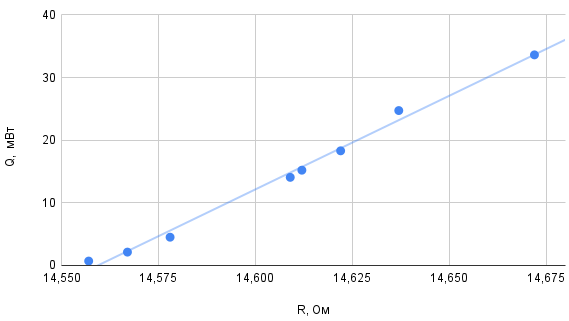
\includegraphics[width=0.7\linewidth]{t=22.png}
    \caption{Зависимость Q от R при $t=22\degree C$}
    \label{fig:my_label}
\end{figure}
\begin{figure}[h]
    \centering
    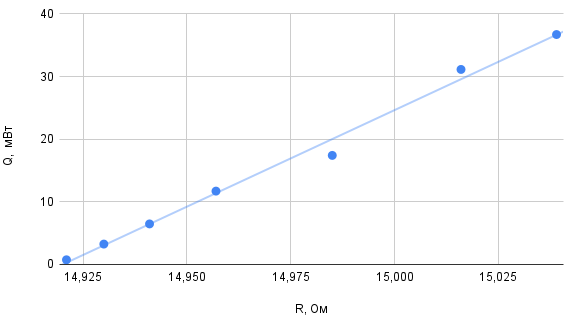
\includegraphics[width=0.7\linewidth]{t=30.png}
    \caption{Зависимость Q от R при $t=30\degree C$}
    \label{fig:my_label}
\end{figure}
\begin{figure}[h]
    \centering
    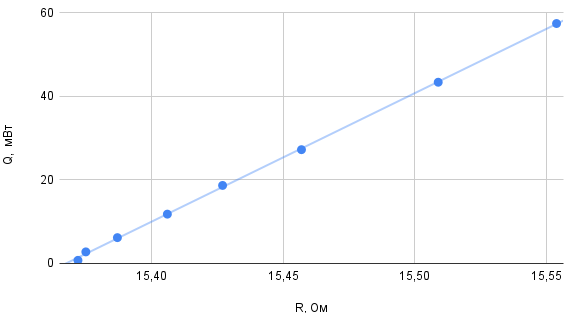
\includegraphics[width=0.7\linewidth]{t=40.png}
    \caption{Зависимость Q от R при $t=40\degree C$}
    \label{fig:my_label}
\end{figure}
\begin{figure}[h]
    \centering
    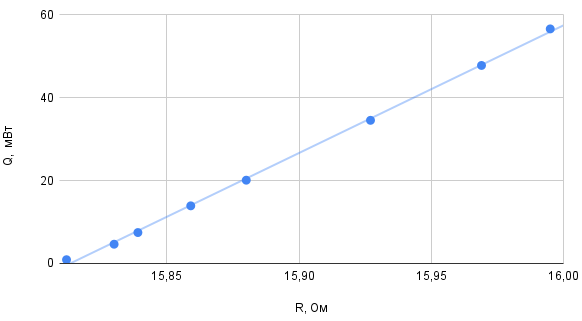
\includegraphics[width=0.7\linewidth]{t=50.png}
    \caption{Зависимость Q от R при $t=50\degree C$}
    \label{fig:my_label}
\end{figure}
\begin{figure}[h]
    \centering
    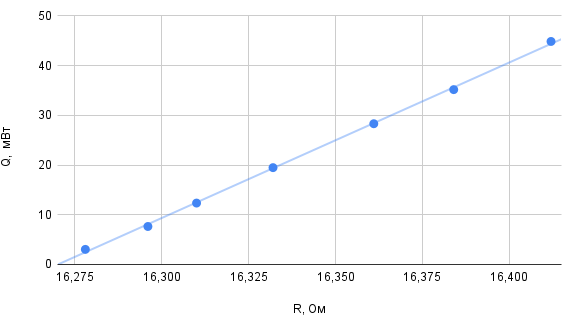
\includegraphics[width=0.7\linewidth]{t=60.png}
    \caption{Зависимость Q от R при $t=60\degree C$}
    \label{fig:my_label}
\end{figure}
\begin{figure}[h]
    \centering
    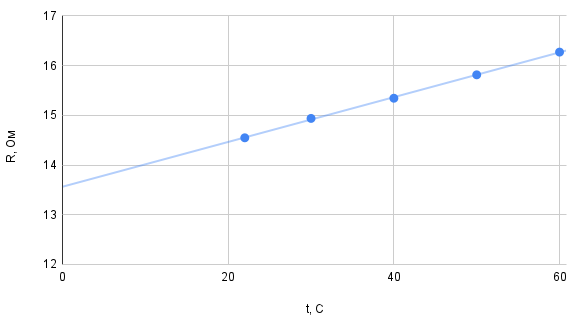
\includegraphics[width=0.7\linewidth]{RTc.png}
    \caption{Зависимость R от t}
    \label{fig:my_label}
\end{figure}
\begin{figure}[h]
    \centering
    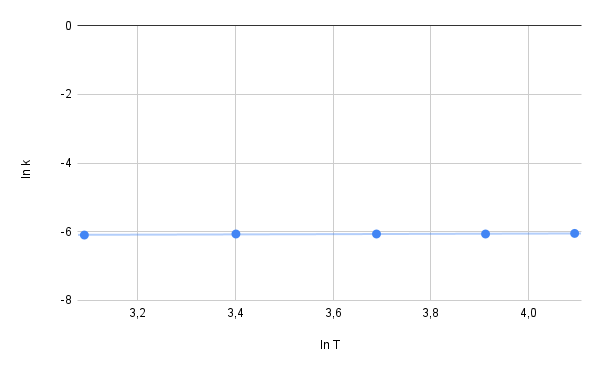
\includegraphics[width=0.7\linewidth]{ln.png}
    \caption{Зависимость ln$\kappa$ от ln$T$}
    \label{fig:my_label}
\end{figure}
\end{document}
